\section{Installation}

\setcounter{equation}{0}

The source code for PFLOTRAN can be downloaded from the bitbucket.org web site using \href{http://mercurial.selenic.com/}{Mercurial} (hg):

\verb|hg clone https://bitbucket.org/pflotran/pflotran-dev|.

This requires first creating a free account on bitbucket.

It should be possible to build and run PFLOTRAN on essentially any system with 
modern C and Fortran (2003 standard or later) compilers and an available 
implementation of the Message Passing Interface (MPI) system that has been 
built with Fortran bindings.
Besides these requirements, the major third-party library required is 
the open-source library PETSc---the Portable, Extensible Toolkit for Scientific 
Computation---that provides the parallel framework on which PFLOTRAN is 
built.
Most of the work involved in building PFLOTRAN lies in building PETSc. 
PETSc uses a sophisticated Python-based build tool, BuildSystem, to perform 
extensive platform discovery and configuration as well as automatic download 
and build for any of the open-source third-party libraries that PETSc can 
use. 
The PFLOTRAN makefiles use the information generated by BuildSystem as part 
of the PETSc build process; once PETSc is built, building PFLOTRAN is  
straightforward.

Besides \href{http://www.mcs.anl.gov/petsc/}{PETSc}, third party libraries commonly installed are
\begin{itemize}
\item MPI, message passing interface (\href{http://www.open-mpi.org/}{OpenMPI} or \href{http://www.mpich.org/}{MPICH})
\item \href{http://www.hdfgroup.org/HDF5/}{HDF5}, required for parallel I/O and reading HDF5-formatted input files
\item \href{http://glaros.dtc.umn.edu/gkhome/views/metis}{Metis} and \href{http://glaros.dtc.umn.edu/gkhome/metis/parmetis/overview}{ParMetis}, graph partitioning libraries required for 
      unstructured grids
\item \href{http://acts.nersc.gov/hypre/}{Hypre}, which provides a variety of preconditioners and multilevel 
      solves
\end{itemize}

PETSc can be used to download, compile and install all of these third party libraries during compilation of PETSc as explained below, so that the user does not have to do this themselves individually for each library.

\subsection{Compilers}

The installation of PFLOTRAN on MacOSX requires compiler versions 4.7 or later for gfortran and gcc to be compatible with Fortran 2003. 

For MacOSX compilers can be obtained from several sources including \href{http://www.macports.org/}{MacPorts} and the web site \href{http://hpc.sourceforge.net/}{High Performance Computing for MacOSX}.

\begin{comment}
\subsection{Mac OS X}

The installation of PFLOTRAN on MacOSX requires compiler versions 4.7.2 or later for gfortran and gcc and must be compatible with object oriented features in Fortran 2003. 
%The compiler g++ is needed for installing SAMRAI.
%Define environment variables: {\tt MPI\_HOME}, {\tt PKGS}, \linebreak {\tt HYPRE\_INSTALL\_DIR}

\subsubsection{OpenMPI}

\begin{verbatim}
setenv F90 gfortran
setenv F77 gfortran
setenv FC gfortran
setenv CC gcc-4
setenv CXX g++-4

./configure \
--prefix=$PKGS/openmpi/openmpi-1.4.1-gcc-4.4.2-gfortran \
--disable-debug \
--enable-static \
--disable-shared

make
make install
\end{verbatim}

\subsubsection{Hypre}

\begin{verbatim}
./configure \
--with-MPI \
--enable-debug \
--disable-opt \
--prefix=${HYPRE_INSTALL_DIR} \
--with-MPI-include=${MPI_HOME}/include \
--with-MPI-libs=openmpi \
--with-MPI-lib-dirs=${MPI_HOME}/lib \
CC=mpicc \
CXX=mpicxx \
F77=mpif90

make
make install
\end{verbatim}
\end{comment}

\subsection{Building PETSc}

The first step to building PFLOTRAN is to configure and build the PETSc 
toolkit.
This requires, at minimum, working installations of C and Fortran 95-compliant 
compilers.
For users looking for an open-source compiler, we recommend the gcc and 
gfortran compilers that are part of the GNU Compiler Collection (GCC), version 
4.7.x or later.
Users may also wish to install MPI and other libraries from source or via a 
package manager, but the PETSc \texttt{./configure} script can be used not only 
to install PETSc but also MPI, HDF5, ParMETIS/METIS, and various solver 
libraries such as MUMPS for sparse direct solvers, Hypre for a variety of 
preconditioners and multi-level solvers, and the Trilinos multilevel solver ML. 
For systems that do not provide specially optimized versions of these 
libraries, we recommend using PETSc's \texttt{configure} to install these 
third-party libraries.
If you do wish to install any of these third-party libraries yourself, you 
will need to do so \textit{before} installing PETSc to that the necessary PETSc 
interfaces to these packages can be built.

The development branch of PFLOTRAN tracks the main development branch of 
PETSc and hence requires this ``petsc-dev'' version, which can be either 
downloaded from the PETSc web page 
\href{http://www.mcs.anl.gov/petsc/developers/index.html}{petsc-dev}, 
or installed using Mercurial following instructions on the PETSc developer web 
page. 
We recommend that PETSc be obtained using the version control system  
(\href{http://mercurial.selenic.com/wiki}{Mercurial}).

Define environment variables $\verb|PETSC_DIR|$ and $\verb|PETSC_ARCH|$ giving the location of the petsc-dev source and the directory where the libraries for the particular architecture are stored after compiling and installing PETSc.

\subsubsection{Mac OS X}

\paragraph{Lion, Mavericks ($\leq$ Mac OS X 10.9.x)} To install ParMETIS/METIS on MacOSX it is necessary to first install the latest version (3.0.x) of CMAKE from e.g. Homebrew, MacPorts or Fink.

To install PETSc, MPI using openmpi, HDF5, and ParMETIS/METIS with debugging turned off configure PETSc using:

\begin{verbatim}
./config/configure.py --with-debugging=0 --with-shared-libraries=0 
--with-x=0 --download-openmpi --download-hdf5=1 
--download-metis=1 --download-parmetis=1
\end{verbatim}

\noindent
followed by

$\verb|make all|$

\noindent
and

$\verb|make test|$

Note that ParMETIS/METIS is only needed for using the unstructured grid capability in PFLOTRAN. HDF5 is recommended for large problems for use with Visit for (parallel) visualization.

\paragraph{Yosemite (Mac OS X 10.10.x)} Special considerations are required to install PETSc and PFLOTRAN on Yosemite (MacOSX 10.10.x). It is necessary to install gcc-4.9 from Homebrew [other installations such as HPC MacOS X are not bug free at the time of this writing (10.23.14)]. The following steps are required:
\begin{enumerate}
\item install Homebrew (standard location /usr/local must be clean to avoid collisions)
\item install gcc (need version 4.9.x): \texttt{brew install gcc}
\item install cmake (need version 3.0.x): \texttt{brew install cmake}
\item configure PETSc using the Mac c and c++ compilers clang, clang++ and gfortran installed from Homebrew: 

$\verb|cd petsc-dev|$\\
\begin{verbatim}
./configure --with-cc=clang --with-cxx=clang++ 
            --with-fc=gfortran --download-mpich=1 
            --download-hdf5=1 --download-metis=1 
            --download-parmetis=1 --with-debugging=0
\end{verbatim} 

\item $\verb|make all|$\\ $\verb|make test|$
%\item $\verb|cd ./pflotran-dev/src/pflotran|$\\ $\verb|make pflotran|$
\end{enumerate}
Notes: At the time of this writing (10.23.14) openmpi did not compile. HDF5 did not compile using gcc-4.9 installed from Homebrew.

\subsubsection{Windows}

To install PETSc and PFLOTRAN on Windows see instructions on the PFLOTRAN wiki \linebreak ({\url{https://bitbucket.org/pflotran/pflotran-dev/wiki/Home}).

\begin{comment}
\subsubsection{MacOSX}

\begin{verbatim}
./config/configure.py \
--with-mpi-dir=$MPI_HOME \
--download-openmpi=1 \
--with-debugging=0 \
--with-shared-libraries=0 \
--download-mumps=1 \
--download-parmetis=1 \
--download-scalapack=1 \
--download-blacs=1 \
--download-ml=1 \
--download-hdf5=1 

make all
make test
\end{verbatim}

\begin{enumerate}
\item Obtain C compiler gcc4.5 or later for snow leopard (e.g. from http://hpc.sourceforge.net). 
%They just had gcc4.6 available recently. 
Install gcc under \verb|/opt/local| or \verb|/usr/local|. 
You don't have to get gcc4.5 or 4.6,
but you have to have a verison not older than gcc4.3 for some features in
pflotran. Both gcc4.5 and gcc4.6 come with gfortran.

\item Install openmpi 1.5.1 from www.open-mpi.org. Configure using the command:

\begin{verbatim}
./configure CC=gcc CXX=g++ FC=gfortran --enable-mpi-f77=no 
--prefix=/opt/local
\end{verbatim}

\item Download petsc-dev and configure using

\begin{verbatim}
./configure --download-hdf5=1 --with-cc=mpicc --with-cxx=mpicxx 
--with-fc=mpif90,
\end{verbatim}

then compile with \verb|make all|.

\item Compile pflotran using

\verb|make pflotran|
\end{enumerate}
\end{comment}

\subsubsection{ORNL's Jaguar XT4/5}

\footnotesize
\begin{verbatim}
./config/configure.py PETSC_ARCH=cray-xt4-pgi_fast \
--configModules=PETSc.Configure \
--optionsModule=PETSc.compilerOptions \
--known-level1-dcache-size=65536 \
--known-level1-dcache-linesize=64 \
--known-level1-dcache-assoc=2 \
--known-memcmp-ok=1 \
--known-sizeof-char=1 \
--known-sizeof-void-p=8 \
--known-sizeof-short=2 \
--known-sizeof-int=4
--known-sizeof-long=8 \
--known-sizeof-long-long=8 \
--known-sizeof-float=4 \
--known-sizeof-double=8 \
--known-sizeof-size_t=8 \
--known-bits-per-byte=8 \
--known-sizeof-MPI_Comm=4 \
--known-sizeof-MPI_Fint=4 \
--known-mpi-long-double=0 \
--with-batch=1 \
--with-shared-libraries=0 \
--with-dynamic=0 \
--with-cc=cc \
--with-cxx=CC \
--with-fc=ftn \
--COPTFLAGS="-tp barcelona-64 -fastsse -Mipa=fast" \
--CXXOPTFLAGS="-tp barcelona-64 -fastsse -Mipa=fast" \
--FOPTFLAGS="-tp barcelona-64 -fastsse" \
--with-debugging=0 \
--with-blas-lib=sci \
--with-lapack-lib=sci \
--with-x=0 \
--with-mpi-dir=$MPICH_DIR \
--download-hypre=1 \
--download-parmetis=1 \
--with-hdf5=1 \
--with-hdf5-dir=$HDF5_DIR \
--known-mpi-shared=0
\end{verbatim}
\normalsize
The user will need to load the following HDF5 module beforehand: \ \verb|module load hdf5-parallel|.

\subsection{Building PFLOTRAN}
 
PFLOTRAN is compiled with the command:

\verb|make [options] pflotran|

\noindent
where several possible options are: 

\begin{tabular}{ll}
Compile Option & \multicolumn{1}{c}{Description}\\
\midrule
%\verb|scco2=1|: & --enable two-phase supercritical CO$_2$ mode\\
\verb|scorpio=1|: & --enable parallel IO\\
\verb|coll=1|: & --enable colloid-facilitated transport option\\
%\verb|temp|: & --enable temperature dependent log $K$ capability\\
%\verb|mfd=1|: & --enable MFD full permeability tensor capability (not operational)
%\verb|ice|:& --enable permafrost hydrology (works only in THC mode)
\end{tabular}

\noindent
See the PFLOTRAN \verb|makefile| for additional options.

\noindent
Compiling in parallel can be achieved using the modified \texttt{make} command:

\verb|make -j # pflotran|

\noindent
where \# denotes the number of cores. A comparison of the speedup possible on Linux-Mint and MacOSX 10.11 is shown in Figure~\ref{fcompile}. The Linux-Mint results are obtained on an 8-core machine; whereas the Mac has 4 cores which could explain the slightly better performance at 8 cores on Linux.

\begin{figure}[h]\centering
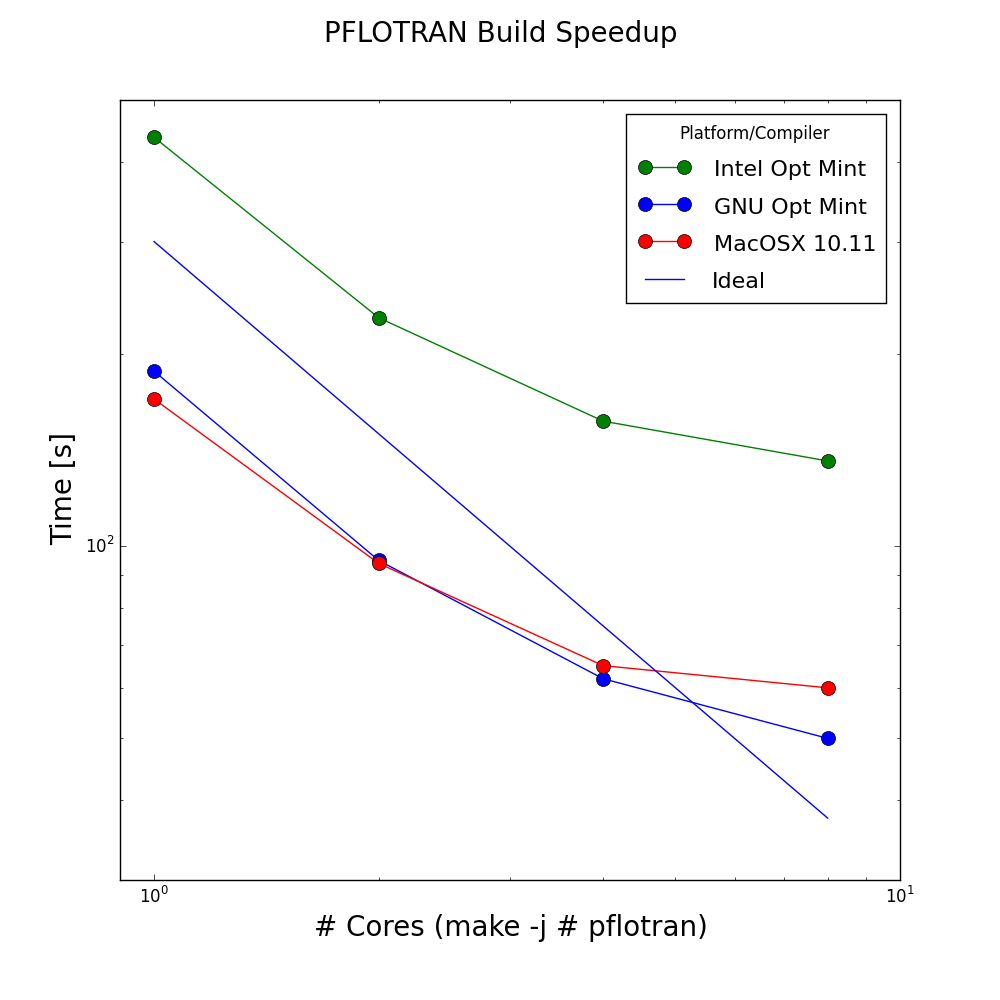
\includegraphics[scale=0.5]{./figs/linux-mac.png}
\caption{Parallel compile time as a function of number of cores for Intel and Gnu compilers on Linux-Mint and the Gnu compiler on MacOSX 10.11. The Mac results are based on gfortran 4.9.1.}
\label{fcompile}
\end{figure}

\subsection{Updating PFLOTRAN}

To update the PFLOTRAN source code
type: 

\texttt{hg pull -u} 

\noindent
from within the PFLOTRAN source repository.
Recompile PFLOTRAN using:

\texttt{make clean}\\
\indent
\texttt{make [options] pflotran}

\subsection{Parallel I/O using Sarat Sreepathi's SCORPIO library with PFLOTRAN}
\label{parallelio}

The SCORPIO (parallel I/O library) enables a scalable general purpose parallel I/O capability for HPC by taking advantage of existing parallel I/O libraries, such as HDF5 which are being widely used by scientific applications, and modifying these algorithms to better scale to larger number of processors. The library has been tested with MPICH-3.0.2 and OpenMPI-1.6.

\normalsize
It is recommended that values for the variables {\footnotesize\tt HDF5\_READ\_GROUP\_SIZE} and \linebreak {\footnotesize\texttt{HDF5\_WRITE\_GROUP\_SIZE}} be set in the input file. 
If they are not set, {\footnotesize\texttt{HDF5\_READ\_GROUP\_SIZE}} is set to total MPI ranks and {\footnotesize\texttt{HDF5\_WRITE\_GROUP\_SIZE}} is set to 1 by default.

Typical values are to set the write group size equal to the number of processes on a compute node (typically 16 or 32). 
%If that still results in a penalty, decrease it further. 
A much higher read group size is preferred, e.g. use 512 when running on 512 cores so that one process reads the input file and broadcasts relevant sections.
Put {\footnotesize\texttt{HDF5\_WRITE\_GROUP\_SIZE}} under the {\footnotesize\texttt{OUTPUT}} keyword:
\footnotesize
\begin{Verbatim}
:=========================== output options ===================================
OUTPUT
  TIMES y 5. 10. 15. 20.
  FORMAT HDF5
  HDF5_WRITE_GROUP_SIZE 16
END
\end{Verbatim}
\normalsize
and {\footnotesize\tt HDF5\_READ\_GROUP\_SIZE} in the main body of the input file:
\footnotesize
\begin{Verbatim}
HDF5_READ_GROUP_SIZE 1024
\end{Verbatim}
\normalsize
% (Sarat: Not necessary) Number of MPI tasks should be an exact multiple of {\footnotesize\tt HDF\_READ\_GROUP\_SIZE}.

For more details on the SCORPIO library, please see Appendix A in Sarat Sreepathi's \linebreak <admin@sarats.com> \href{http://www.lib.ncsu.edu/resolver/1840.16/8317}{dissertation}.

Instructions for downloading and installing the SCORPIO library for use with PFLOTRAN is provided below. Note that this software is separate from PFLOTRAN and under a LGPL.
\begin{enumerate}

\item Download source code for building the SCORPIO library:

{\small\texttt{svn co http://ascem-io.secure-water.org/ascem-io/scorpio DIRNAME}}

where {\footnotesize\texttt{DIRNAME}} is the installation directory (Default: {\footnotesize\texttt{scorpio}}). 

The username and password are:
%\href{https://bitbucket.org/pflotran/pflotran-dev/wiki/Documentation/Strata}{Strata}

username: {\footnotesize\texttt{pflotran\_dev}}

password: {\footnotesize\texttt{gr0undw@t3r}}

\item Compile SCORPIO library:
First, set the environment variable {\footnotesize\tt SCORPIO\_DIR} to a directory where you wish to install the library files. 
Please make sure that you have the correct permissions to write to that location. For example, you can use something like \linebreak {\footnotesize\tt \$\{HOME\}/parallelIO/scorpio}.
Depending on the shell you are using you may use:

\footnotesize {\tt export SCORPIO\_DIR=<your-iolib-install-dir>} \hfill {\it (bash shell)}
\normalsize

or

\footnotesize
{\tt setenv SCORPIO\_DIR <your-iolib-install-dir>} \hfill {\it (tcsh/csh shell)}

\normalsize

To compile the library, check to make sure that the Makefile has the right settings for your machine.
Typically, the current configuration suffices. So you can just follow the instructions below.
For advanced users, please edit the section for {\footnotesize\tt pflotran\_machine} in the Makefile as desired.
% So just uncomment the line {\small\tt MACHINE=pflotran\_machine}.
% \footnotesize
% \begin{Verbatim}
% 66 # Note: PFLOTRAN USERS: Make sure to uncomment line below 
%    OR use make MACHINE=pflotran_machine
% 67 MACHINE=pflotran_machine
% ...
% 73 ifeq ($(MACHINE),pflotran_machine)
% 74     CC=${PETSC_DIR}/${PETSC_ARCH}/bin/mpicc
% 75     FC=${PETSC_DIR}/${PETSC_ARCH}/bin/mpif90
% 76     LINKER=${FC}
% 77     CFLAGS+= -I${PETSC_DIR}/${PETSC_ARCH}/include -O3
% 78     FFLAGS+= -I${PETSC_DIR}/${PETSC_ARCH}/include -O3 
% 79     LDFLAGS+= -Wl,-L${PETSC_DIR}/${PETSC_ARCH}/lib -lhdf5 -lz 
% 80 endif
% \end{Verbatim}

This assumes that you have let PETSc build MPI and {\tt mpicc} and {\tt mpif90} are located in \linebreak \verb|${PETSC_DIR}/${PETSC_ARCH}/bin|. If not, you may need to alter the {\tt Makefile} to provide the correct path to the location of the MPI compilers.

\footnotesize
{\tt cd DIRNAME/src}


{\tt make MACHINE=pflotran\_machine}

{\tt make install} \hfill {\it (compile with {\tt mpicc})}
\normalsize

This will build the library {\footnotesize\tt libscorpio.a} and copy corresponding files to {\footnotesize\tt SCORPIO\_DIR/lib} and {\footnotesize\tt SCORPIO\_DIR/include} directories.

On machines with MPI installed modify the makefile to use the native {\tt mpi} compilers:
\footnotesize
\begin{Verbatim}
ifeq ($(MACHINE),pflotran_machine)
  CC=mpicc
  FC=mpif90
  LINKER=${FC}
  CFLAGS+= -I${PETSC_DIR}/${PETSC_ARCH}/include -O3
  FFLAGS+= -I${PETSC_DIR}/${PETSC_ARCH}/include -O3 
  LDFLAGS+= -Wl,-L${PETSC_DIR}/${PETSC_ARCH}/lib -lhdf5 -lz 
endif
\end{Verbatim}
\normalsize

\item Compile PFLOTRAN:

Please ensure that environmental variable: {\footnotesize\tt SCORPIO\_DIR} is pointed to \linebreak {\footnotesize\tt <your-iolib-install-dir>}:

{\footnotesize\tt cd PFLOTRAN\_DIR/src/pflotran}

{\footnotesize\tt make scorpio=1 pflotran}
\normalsize
\end{enumerate}

\scriptsize
\begin{verbatim}
-------------------------------------------------------------------------------
SCORPIO
Scalable Parallel I/O module for Environmental Management Applications
-------------------------------------------------------------------------------
This library provides software that read/write data sets from/to parallel file 
systems in an efficient and scalable manner. 
In this context, scalable means that the simulators read/write 
performance does not degrade significantly as the number of cores grows.

-------------------------------------------------------------------------------
COPYRIGHT AND LICENSE 
-------------------------------------------------------------------------------
SCORPIO is distrubuted under the terms of the GNU Lesser General Public 
License (LGPL). The copyright is held jointly by North Carolina State University 
and Pacific Northwest National Laboratory. 

The copyright and license information is specified in the included file 
COPYRIGHT. 

-------------------------------------------------------------------------------
Repository Access
-------------------------------------------------------------------------------
Please request write access by contacting Kumar Mahinthakumar (gmkumar@ncsu.edu). 
Use the following command to access repository:
	svn co http://ascem-io.secure-water.org/ascem-io

-------------------------------------------------------------------------------
Building Library
-------------------------------------------------------------------------------
The current stable release is 2.2.

--------------
Prerequisites:
--------------
MPI
C compiler
HDF5 libraries (preferably with parallel(MPI) support)
Optional: Fortran (for Fortran example)

After downloading SCORPIO and gathering details of HDF5 installation, 
the following commands can be used to build and install SCORPIO: 

	cd <SCORPIO check out directory>/src
	make CC=<C-compiler> HDF5_INCLUDE_DIR=<location of the HDF5 include directory>
	make SCORPIO_INSTALL_DIR=<user defined install location> install

In this case, CC refers to C compiler with MPI support, e.g., mpicc.

-------------------------------------------------------------------------------
\end{verbatim}

\normalsize

\newpage
\subsection{Running PFLOTRAN}

PFLOTRAN can be run from the command line as

\verb|mpirun -np 10 pflotran [options]|

A number of command line options are available:

\begin{tabular}{lp{9cm}}
\toprule
Option & \multicolumn{1}{c}{Description}\\
\midrule
{\tt -pflotranin <string>} & specify input file [Default: {\tt pflotran.in}]\\
{\tt -input\_prefix <string>} & specify input file prefix and path [default: {\tt pflotran}]\\
{\tt -output\_prefix <string>} & specify output file prefix and path to prefix directory which must already exist [default: {\tt pflotran}]\\
{\tt -screen\_output off} & turn off screen output\\
%{\tt -v} &\\
{\tt -realization\_id <integer>} & run specified realization ID\\
{\tt -multisimulation} & run multiple input files in one run\\
{\tt -stochastic} & Monte Carlo multiple realization run\\
\midrule
\multicolumn{2}{c}{PETSc}\\
\midrule
{\tt -help} & print list of command line options\\
{\tt -log\_view} & print out PETSc run performance\\
{\tt -snes\_converged\_reason} & print the reason for convergence/divergence after each solve\\
{\tt -on\_error\_abort} & aborts run on hitting NaNs\\
\texttt{-no\_signal\_handler} & turn off PETSc error handling\\
{\tt -v} & <int> verbose\\
{\tt -options\_left} & for debugging: lists any PETSc objects that have not been freed\\
{\tt -snes\_monitor} & print to screen function norm with each iteration\\
{\tt -snes\_linesearch\_monitor} & print to screen line search information\\
{\tt -snes\_view} & print line search method\\
{\tt -snes\_ls} & options: [cubic, quadratic, basic, basicnonorms] \\
{\tt -snes\_type newtonls} & \\
{\tt -snes\_type newtontr} & \\
{\tt -snes\_tr\_delta0} & <delta0>\\
{\tt -snes\_monitor\_lg\_residualnorm} & draws line graph of the residual norm convergence using X11\\
{\tt -ksp\_monitor\_lg\_residualnorm} & \\
\bottomrule
\end{tabular}

\begin{mdframed}
\textbf{Examples:}

\verb|mpirun -np 1 ./pflotran -output_prefix ./path_to/prefix|\\
\end{mdframed}


\subsection{Multiple Realization Simulation Mode}

To launch 1000 realizations on 100 processor groups using 10,000 processor cores:

\noindent
\texttt{mpirun -np 10000 pflotran -stochastic -num\_realizations 1000 \linebreak 
-num\_groups 100}

\noindent
Each processor group will utilize 100 processor cores and run 10 realizations apiece \linebreak (\texttt{num\_realizations/num\_groups}), one after another. Thus, 100 realizations are executed simultaneously with each processor group simulating a single realization on 100 processor cores at a time. Each processor group continues to run realizations until its allocation of 10 is completed.

\noindent
To simulate a specific realization without running in multi-realization stochastic mode use:

\texttt{mpirun -np 10000 pflotran -realization\_id <integer>}

\noindent
where <integer> specifies the realization id.

\subsection{Multiple Simulation Mode}

To run multiple input decks simultaneously, create a file e.g. \texttt{filenames.in}, containing the list of filenames that are to be run:
\begin{Verbatim}
                             sim1.in
                             sim2.in
                             ...
                             sim100.in
\end{Verbatim}
where \texttt{simn.in} is the usual PFLOTRAN input file. The names may be arbitrarily chosen. Then, launch the run as:

\verb|mpirun -n XXX pflotran -pflotranin filenames.in -multisimulation| 

\noindent  
Note that all simulations run at once. The same logic used to allow a processor group to run multiple simulations with \texttt{multirealization} is {\em not} implemented. \textbf{Choose the number of cores to be a multiple of the number of input filenames listed in the input file (i.e. filenames.in).} All output files have \texttt{Gn} appended to the file name, e.g. \texttt{sim10G10-001.tec}.

%%%%%%%%%%%%%%%%%%%%%%%%%%%%%%%%%%%%%%%%%%%%%%%%%%%%%%%%%%%%%%%%%%%%%%%%%%%
\begin{comment}
\subsection{Building SAMRAI Version 2.4.4}

\noindent
To build SAMRAI follow the instructions listed below.

{\tt mkdir SAMRAI-v2.4.4}

{\tt cd SAMRAI-v2.4.4}

{\tt hg clone http://software.lanl.gov/pflotran/hg/samrai SAMRAI}

{\tt mkdir samrai-objs in directory SAMRAI-v2.4.4}

{\tt cd samrai-objs}

Define the environment variables $\verb|SAMRAI_INSTALL_DIR|$, $\verb|MPI_HOME|$, $\verb|HDF5_HOME|$, \linebreak $\verb|PETSC_DIR|$ to be the top level directories of the appropriate packages

\noindent
With MPICH:
\begin{verbatim}
../SAMRAI/configure --prefix=${SAMRAI_INSTALL_DIR} \
--with-CC=mpicc \
--with-CXX=mpicxx \
--with-F77=mpif90 \
--with-mpi \
--with-mpi-include=${MPI_HOME}/include \
--with-mpi-lib-dirs=${MPI_HOME}/lib \
--with-MPICC=mpicc \
--with-x \
--with-hdf5=${HDF5_HOME} \
--with-hypre=${HYPRE_HOME} \
--with-petsc=${PETSC_DIR} \
--with-blaslapack \
--enable-opt \
 --enable-debug \
--enable-char \
--enable-bool \
CXXFLAGS="-DMPICH_IGNORE_CXX_SEEK -DMPICH_SKIP_MPICXX" \
CPPFLAGS="-DMPICH_IGNORE_CXX_SEEK -DMPICH_SKIP_MPICXX"
\end{verbatim}

\noindent
With OPENMPI:
\begin{verbatim}
../${SAMRAI_SRC_DIR}/configure \
--prefix=${SAMRAI_INSTALL_DIR} \
--with-CC=mpicc \
--with-CXX=mpicxx \
--with-F77=mpif90 \
--with-mpi \
--with-mpi-include=${MPI_HOME}/include 
--with-mpi-lib-dirs=${MPI_HOME}/lib 
--with-MPICC=mpicc \
--with-x \
--with-hdf5=${HDF5_INSTALL_DIR} \
--with-hypre=${HYPRE_INSTALL_DIR} \
--with-petsc=${PETSC_DIR} \
--with-blaslapack \
--disable-opt \
--enable-debug \
--enable-char \
--enable-bool \
CXXFLAGS="-DOMPI_IGNORE_CXX_SEEK -DOMPI_SKIP_MPICXX \
  -I${PETSC_DIR}/${PETSC_ARCH}/include -I${PETSC_DIR}/include" \
CPPFLAGS="-DOMPI_IGNORE_CXX_SEEK -DOMPI_SKIP_MPICXX"
\end{verbatim}

{\tt make}

{\tt make install}

Define the environment variable $\verb|SAMRAI|$ to point to $\verb|SAMRAI_INSTALL_DIR|$ (for example in your .cshrc)

Instructions for SAMR utils package

{\tt hg clone  http://software.lanl.gov/pflotran/hg/samrutils}

{\tt cd samrutils}

Define the environment variable $\verb|AMRUTILITIES_HOME|$ to be the directory where you want the libraries and headers installed, it can point to the top level src dir if you like.

\verb|make prefix=${AMRUTILITIES_HOME} lib3d|

Instructions for SAMR solvers package

{\tt hg clone  http://software.lanl.gov/pflotran/hg/samrsolvers}

{\tt cd samrsolvers}

Define the environment variable $\verb|SAMRSOLVERS_HOME|$ to be the directory where you want the libraries and headers installed, it can point to the top level src dir if you like.

\verb|make prefix=${SAMRSOLVERS_HOME} lib3d|

\noindent
Assumptions:
\begin{enumerate}
\item External packages needed by PFLOTRAN are built: petsc-dev, hypre,  
hdf5, \linebreak mpich2/openmpi/some mpi
\item External packages needed by PFLOTRAN AMR interface are built:  
SAMRAI, SAMRUtils, SAMRSolvers
\end{enumerate}

\noindent
Define the environment variables:
\begin{center}
\begin{tabularx}{\linewidth}{lX}
\bf SAMRAI &--points to where SAMRAI is installed\\
\bf AMRUTILITIES\_HOME &--points to where SAMRUtils is installed\\
\bf SAMRSOLVERS\_HOME &--points to where SAMRSolvers is installed
\end{tabularx}
\end{center}

\noindent
Instructions for building $\verb|SAMRAIDriver|$:
\begin{center}
\begin{verbatim}
cd pflotran/src/pflotran
make samr_hdf5=1 pflotranamr

cd samr/src
make
\end{verbatim}
\end{center}

\noindent
At this point there should exist an executable named SAMRAIDriver.

\subsubsection{Running PFLOTRAN/SAMRAI on Jaguar}

Add to the {\tt .tcshrc} (or equivalent) file:
\begin{verbatim}
umask 0002
set LD_LIBRARY_PATH=/usr/lib64:${LD_LIBRARY_PATH}
setenv ARCH cray-xt5
setenv COMPILER gcc-4.4.2
setenv OPT opt
#setenv OPT debug 
setenv PROJ_DIR /tmp/proj/csc025/csc025geo3
setenv PKGS ${PROJ_DIR}/packages
setenv PKG_POSTFIX ${ARCH}-${COMPILER}-${OPT}
setenv PETSC_ARCH ${PKG_POSTFIX} 
setenv PETSC_VERSION petsc-dev
setenv PETSC_DIR ${PKGS}/petsc/${PETSC_VERSION}-${OPT}
setenv SAMRAI ${PKGS}/samrai/SAMRAI-v2.4.4/${PETSC_VERSION}-${PKG_POSTFIX}
setenv AMRUTILITIES_HOME ${PKGS}/samrutils/${PKG_POSTFIX}
setenv SAMRSOLVERS_HOME ${PKGS}/samrsolvers/${PKG_POSTFIX}
setenv PCH ${SAMRSOLVERS_HOME} 
 
setenv MPICH_UNEX_BUFFER_SIZE 400M
setenv MPICH_PTL_OTHER_EVENTS 4096
setenv MPICH_PTL_SEND_CREDITS -1
setenv MPICH_MSGS_PER_PROC 60000
\end{verbatim}

\noindent
Load the following modules:
\begin{verbatim}
module swap PrgEnv-pgi PrgEnv-gnu
 
module load mercurial
module load hdf5-parallel/1.8.3.1
module load hypre/2.4.0b
module load szip/2.1
module load totalview/8.6.0-1
\end{verbatim}

%########################################################################

\noindent
The user will need to set: PETSC\_DIR, PETSC\_ARCH, AMRUTILITIES\_HOME, SAMRSOLVERS\_HOME
to be defined as above. Also, note the swap to gnu.
\begin{verbatim}
 
cd pflotran
hg pull -u

cd src/pflotran
make hdf5=1 jaguar=1 pflotranamr

cd samr/src
make hdf5=1 jaguar=1
\end{verbatim}
At this point you should have an executable \verb|SAMRAIDriver|.
 
%\noindent
%To run the code do:

%\noindent
%\verb|cd nmg.4320|\\
%\verb|qsub run.4320|
 
%\noindent
%This should run the coupled flow (richards) and transport (15 species).

\end{comment}
%%%%%%%%%%%%%%%%%%%%%%%%%%%%%%%%%%%%%%%%%%%%%%%%%%%%%%%%%%%%%%%%%%%%%%%%%%%

%%%%%%%%%%%%%%%%%%%%%%%%%%%%%%%%%%%%%%%%%%%%%%%%%%%%%%%%%%%%%%%%%%%%%%%%%%%
\begin{comment}
The following instructions should aid in installing openmpi, PETSc, HDF5 and PFLOTRAN on a UNIX or Mac computer running MacOSX 10.4 or later.

\subsection{Openmpi}

Set environment variables \verb|PKGS| and \verb|MPI_HOME| and the appropriate \verb|PATH|:

\verb|setenv PKGS /Users/lichtner/petsc/packages|

\verb|setenv MPI_HOME $PKGS/openmpi/openmpi-1.2.5-gcc-4.0.1-absoft-10.1|

\verb|setenv PATH \$PKGS/openmpi/openmpi-1.2.5-gcc-4.0.1-absoft-10.1:\$PATH|

\verb|setenv F90 f90|

\verb|setenv F77 'f90 -YEXT_NAMES=LCS -YEXT_SFX= -f'|

\verb|setenv FC 'f90 -YEXT_NAMES=LCS -YEXT_SFX= -f'|

\verb|setenv CC gcc|

\noindent
Configure using:

\verb|./configure --prefix=$PKGS/openmpi/openmpi-1.2.6-gcc-4.0.1-absoft-10.1|

\noindent
Finally, compile, check installation and install:

\verb|make|

\verb|make check|

\verb|make install|

\subsection{PETSc}

PFLOTRAN uses the Developer version of PETSc. To install PETSc first set the enviroment variables \verb|PETSC_DIR| and \verb|PETSC_ARCH|:

\verb|setenv PETSC_DIR /Users/lichtner/petsc/petsc-dev|

\verb|setenv PETSC_ARCH Intel_MacOSX10.5|

\noindent
Configure PETSc on a Mac using openmpi and Fortran 90 Absoft 10.1:
\begin{verbatim}
./config/configure.py
--with-blas-lapack-lib="-framework vecLib"
--with-mpi-dir=$PKGS/openmpi/openmpi-1.2.6-gcc-4.0.1-absoft-10.1
--with-debugging=0
--with-shared=0
\end{verbatim}

\noindent
Compile and test the PESTc installation with:

\verb|make all test|

\noindent
Optionally install PETSc:

\verb|make install|


\subsection{HDF5}

To install HDF5 set the following environment variables:

\verb|setenv HDF5_INCLUDE $PKGS/hdf/hdf5-1.6.7-gcc-4.0.1-absoft-10.1/include|

\verb|setenv HDF5_LIB $PKGS/hdf/hdf5-1.6.7-gcc-4.0.1-absoft-10.1/lib|

\verb|setenv CC $MPI_HOME/bin/mpicc|

\verb|setenv F9X $MPI_HOME/bin/mpif90|

\verb|setenv CFLAGS -fno-strict-aliasing|

\verb|setenv FFLAGS ""|

\begin{verbatim}
./configure --enable-fortran
--prefix=$PKGS/hdf/hdf5-1.6.7-gcc-4.0.1-absoft-10.1
--disable-debug --enable-production --enable-parallel
--enable-static --disable-shared
\end{verbatim}

\verb|make|

\verb|make check|

\verb|make install|

\subsection{PFLOTRAN}

Compile PFLOTRAN using the command

\verb|make [hdf5=1] pflotran|

\noindent
Create input file \verb|pflotran.in| and run PFLOTRAN with the command:

\verb|mpirun -np #proc pflotran|

\noindent
where \verb|#proc| is the desired number of processor cores.

%%%%%%%%%%%%%%%%%%%%%%%%%%%%%%%%%%%%%%%%%%%%%%%%%%%%%%%%%%%%%%%%%%%%%

\subsection{Direct Solvers}

To implement direct solvers in PETSc with PFLOTRAN first recompile PETSc with the options (petsc-dev, MacOSX 10.5):

\begin{verbatim}
./config/configure.py --with-blas-lapack-lib="-framework vecLib"
--with-mpi-dir=\$PKGS/openmpi/openmpi-1.2.7-gcc-4.0.1-absoft-10.1
--with-debugging=0 --with-shared=0
--download-mumps=1
--download-parmetis=1 --with-parmetis
--download-scalapack=1 --with-scalapack
--download-blacs=1 --with-blacs
\end{verbatim}

\noindent
Then run PFLOTRAN with the command-line options:
\begin{verbatim}
-flow\_mat\_type mpiaij
-flow\_ksp\_type preonly
-flow\_pc\_type lu
-flow\_pc\_factor\_mat\_solver\_package mumps
\end{verbatim}

\subsection{Trilinos}

The Trilinos package for multi-level solvers (ML) may be used with PETSc by configuring petsc-dev with the flag

\begin{verbatim}
./config/configure.py ... --download-ml
\end{verbatim}

When running PFLOTRAN add \verb|-flow_pc_type ml| and/or \verb|-trans_pc_type ml|.
ML options are given in the manual page for PCML (not tested).

\subsection{Condition Number of the Preconditioned Jacobian Matrix}

Since the preconditioned matrix is not explicitly computed, it is necessary to estimate the condition number of the preconditioned Jacobian matrix using PETSc during a PFLOTRAN run. To do this specify a KSP type of GMRES (the Hessenberg matrix is needed that is constructed as part of the Arnoldi process), and then specify

 \texttt{-ksp\_monitor\_singular\_value}

The ratio of the largest to smallest singular values gives the condition number estimate for the preconditioned operator.  Note that this flag will also cause the 2-norm of the true residual (as opposed to the preconditioned residual) to be printed.

If you are doing this in the current version of PFLOTRAN, you need

 \texttt{-flow\_ksp\_type gmres -flow\_ksp\_monitor\_singular\_value}

The estimates will get better the closer one is to the GMRES restart.  (When restart occurs, the Hessenberg matrix from which the eigenvalue estimates are obtained gets discarded along with everything else.)  The frequency can be changed via the option

 \texttt{-flow\_ksp\_gmres\_restart <positive integer>}

The default restart frequency is 30.
\end{comment}
%%%%%%%%%%%%%%%%%%%%%%%%%%%%%%%%%%%%%%%%%%%%%%%%%%%%%%%%%%%%%%%%%%%%%%%%%%%
